\subsection{First simulation study}\label{sim1}

In this study, the performance of a traditional and the new
compartmental model is compared by assessing the accuracy with
which both models determine the time course of the somal potential
of the test neuron (Figure \ref{TestNeuron}) when the neuron is
subjected to large scale exogenous point input. Each simulation
distributes 75 point inputs at random over the dendritic tree of
the test neuron, where each input has strength
$2\times10^{-5}\,\mu$A. These inputs are then mapped to positions
on the Rall equivalent cylinder at the same electrotonic distance
from the soma (assumed to be a sphere of diameter $40\,\mu$m). The
time course of the potential at the soma of the equivalent
cylinder due to the combined effect of these inputs is determined
analytically and taken to be the reference potential against which
error in both compartmental models is measured. The difference
between a computed potential and its exact value is determined at
one millisecond intervals in the first 10 milliseconds of the
simulation, and each difference is divided by the exact potential
at that time to get a relative measure of error. The simulation
procedure is repeated 2000 times to determine the statistics of
the relative error for each of 13 different levels of spatial
discretisation (number of compartments).

\subsubsection{Results}

The results for this study are set out in Table \ref{simex1}. This
table shows the common logarithms of the mean value of the modulus
of the relative error and the standard deviation of that error
estimated ten milliseconds after the initiation of the stimulus.
Similar results (not shown) hold for all times at which the errors
were estimated.

\begin{table}[!h]
\[
\begin{array}{c|cc|cc}
\hline
\mbox{\begin{tabular}{c} Compartments \\[-5pt]
(log$_{10}(\mbox{Compartments}))$ \end{tabular}} &
\multicolumn{2}{|c|}{\mbox{\begin{tabular}{cc}
Traditional & New Model \\[-5pt] \multicolumn{2}{c}{$\log_{10}$(Mean)}
\end{tabular}}}
& \multicolumn{2}{|c}{\mbox{\begin{tabular}{cc}
Traditional & New Model \\[-5pt]
\multicolumn{2}{c}{$\log_{10}$(Standard Dev.)} \end{tabular}}}\\
\hline
\phantom{0}17 \quad (1.2305) & -2.41151 & -2.71945 & -2.62290 & -3.19338 \\
\phantom{0}21 \quad (1.3222) & -2.47233 & -2.77674 & -2.69851 & -3.24583 \\
\phantom{0}34 \quad (1.5314) & -2.94299 & -3.41196 & -3.06731 & -3.88820 \\
\phantom{0}41 \quad (1.6127) & -3.04729 & -3.62138 & -3.17081 & -4.14997 \\
\phantom{0}54 \quad (1.7323) & -3.21258 & -3.89150 & -3.34889 & -4.41251 \\
\phantom{0}61 \quad (1.7853) & -3.24692 & -3.91268 & -3.37653 & -4.45051 \\
\phantom{0}75 \quad (1.8750) & -3.35180 & -4.12056 & -3.46881 & -4.65463 \\
\phantom{0}82 \quad (1.9138) & -3.39846 & -4.23567 & -3.51591 & -4.76498 \\
\phantom{0}93 \quad (1.9684) & -3.45602 & -4.30636 & -3.57633 & -4.82045 \\
          193 \quad (2.2855) & -3.77417 & -4.94731 & -3.89829 & -5.47886 \\
          293 \quad (2.4668) & -3.94409 & -5.31876 & -4.07811 & -5.84771 \\
          390 \quad (2.5910) & -4.08234 & -5.57349 & -4.20025 & -6.10791 \\
          495 \quad (2.6946) & -4.15996 & -5.78252 & -4.28525 & -6.32790 \\
\hline
\end{array}
\]
\centering
\parbox{5in}{\caption{\label{simex1} The result of 2000 simulations
for each of 13 different levels of discretisation used in the
implementation of a traditional and new compartmental model. The
common logarithms of the mean value of the modulus of the relative
error and the standard deviation of that error are estimated at
ten milliseconds after the initiation of the stimulus.}}
\end{table}

The left hand panel of Figure \ref{mean} shows regression lines of
the common logarithms of the modulus of the mean relative error
(denoted by $\overline{RE\phantom{\vert\hskip-4pt}}\;$) for the
traditional (dashed line) and new (solid line) compartmental
models on the logarithm of the number of compartments (denoted by
$N$) used to represent the model neuron. These lines, based on the
data in Table \ref{simex1}, have equations
\begin{equation}\label{mean1}
\begin{array}{rcl}
\log_{10}\overline{RE\phantom{\vert\hskip-4pt}}_\mathrm{\,\small
traditional} & = & -1.09-1.17\log_{10}N\,, \\[5pt]
\log_{10}\overline{RE\phantom{\vert\hskip-4pt}}_\mathrm{\,\small
new} & = & -0.17-2.10\log_{10}N
\end{array}
\end{equation}
in which the regressions are achieved with adjusted $R^2$
values\footnote{$R^2$ measures the proportion of the total
variation of the dependent variable about its mean value that is
explained by the regression, and necessarily takes a value between
zero and one expressed as a percentage.} of $97.4\%$ and $99.5\%$
respectively. In view of the very high $R^2$ values for these
regression equations, a number of conclusions can be drawn from
this simulation study. For a fixed number of compartments, the
error in the new compartmental model is always less than that of
the traditional model. The regression equations (\ref{mean1})
support the argument made in Section \ref{assertion} that the
error in a traditional compartmental model in the presence of
exogenous point current input is approximately $O(1/n)$, whereas
the comparable error in the new compartmental model is
approximately $O(1/n^2)$. In practical terms, for example, the
regression results (\ref{mean1}) suggest that the new
compartmental model with 100 compartments achieves approximately
the same level of accuracy as a traditional model with 500
compartments.

\begin{figure}[!h]
\centerline{\includegraphics[ ]{NCFig5a.eps}
\quad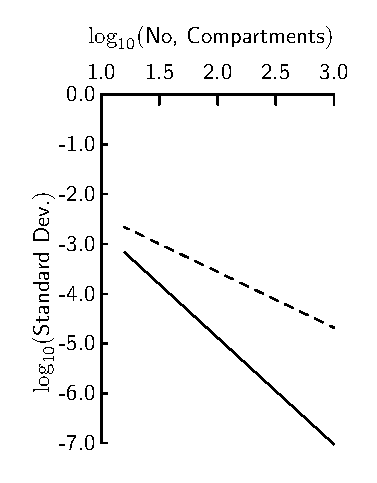
\includegraphics[ ]{NCFig5b.eps}}
\centering
\parbox{5.2in}{\caption{\label{mean} The left panel shows the
regression lines of the common logarithm of the mean relative
errors in the new compartmental model (solid line) and a
traditional compartmental model (dashed line) against the common
logarithm of the number of compartments. All errors are measured
ten milliseconds after initiation of the stimulus. The right panel
shows the regression lines for the standard deviations of the mean
relative errors for the new compartmental model (solid line) and
for a traditional compartmental model (dashed line).}}
\end{figure}

%\begin{figure}[!h]
%\centerline{\begin{mfpic}[56][24]{0.4}{3}{-7.5}{1}
%\headlen7pt
%\pen{1pt}
%\dotspace=4pt
%\dotsize=1.5pt
%%
%% x-axis
%\tlabel[br](3.0,0.9){\textsf {$\log_{10}(\mbox{No. Compartments})$}}
%\lines{(1.0,0),(3.0,0)}
%\lines{(1.5,0),(1.5,-0.2)}
%\lines{(2.0,0),(2.0,-0.2)}
%\lines{(2.5,0),(2.5,-0.2)}
%\lines{(3.0,0),(3.0,-0.2)}
%\tlabel[bc](1.0,0.3){\textsf{1.0}}
%\tlabel[bc](1.5,0.3){\textsf{1.5}}
%\tlabel[bc](2.0,0.3){\textsf{2.0}}
%\tlabel[bc](2.5,0.3){\textsf{2.5}}
%\tlabel[bc](3.0,0.3){\textsf{3.0}}
%% y-axis
%\tlabel[bc](0.5,-6){\rotatebox{90}{\textsf{$\log_{10}(\mbox{Mean relative error})$}}}
%\lines{(1,0),(1,-7)}
%\lines{(1.0,-1.0),(1.05,-1.0)}
%\lines{(1.0,-2.0),(1.05,-2.0)}
%\lines{(1.0,-3.0),(1.05,-3.0)}
%\lines{(1.0,-4.0),(1.05,-4.0)}
%\lines{(1.0,-5.0),(1.05,-5.0)}
%\lines{(1.0,-6.0),(1.05,-6.0)}
%\lines{(1.0,-7.0),(1.05,-7.0)}
%\tlabel[cr](0.95,-0.0){\textsf{0.0}}
%\tlabel[cr](0.95,-1.0){\textsf{-1.0}}
%\tlabel[cr](0.95,-2.0){\textsf{-2.0}}
%\tlabel[cr](0.95,-3.0){\textsf{-3.0}}
%\tlabel[cr](0.95,-4.0){\textsf{-4.0}}
%\tlabel[cr](0.95,-5.0){\textsf{-5.0}}
%\tlabel[cr](0.95,-6.0){\textsf{-6.0}}
%\tlabel[cr](0.95,-7.0){\textsf{-7.0}}
%%
%% Mean values at t=10
%\dashed\lines{(1.2,-2.494),(3.0,-4.60)}
%\lines{(1.2,-2.686),(3.0,-6.466)}
%\end{mfpic}
%\begin{mfpic}[56][24]{0}{3}{-7.5}{1}
%\headlen7pt
%\pen{1pt}
%\dotspace=4pt
%\dotsize=1.5pt
%%
%% x-axis
%\tlabel[br](3.0,0.9){\textsf{$\log_{10}(\mbox{No, Compartments})$}}
%\lines{(1.0,0),(3.0,0)}
%\lines{(1.5,0),(1.5,-0.2)}
%\lines{(2.0,0),(2.0,-0.2)}
%\lines{(2.5,0),(2.5,-0.2)}
%\lines{(3.0,0),(3.0,-0.2)}
%\tlabel[bc](1.0,0.3){\textsf{1.0}}
%\tlabel[bc](1.5,0.3){\textsf{1.5}}
%\tlabel[bc](2.0,0.3){\textsf{2.0}}
%\tlabel[bc](2.5,0.3){\textsf{2.5}}
%\tlabel[bc](3.0,0.3){\textsf{3.0}}
%% y-axis
%\tlabel[bc](0.5,-6){\rotatebox{90}{\textsf{$\log_{10}(\mbox{Standard Dev.})$}}}
%\lines{(1,0),(1,-7)}
%\lines{(1.0,-1.0),(1.05,-1.0)}
%\lines{(1.0,-2.0),(1.05,-2.0)}
%\lines{(1.0,-3.0),(1.05,-3.0)}
%\lines{(1.0,-4.0),(1.05,-4.0)}
%\lines{(1.0,-5.0),(1.05,-5.0)}
%\lines{(1.0,-6.0),(1.05,-6.0)}
%\lines{(1.0,-7.0),(1.05,-7.0)}
%\tlabel[cr](0.95,-0.0){\textsf{0.0}}
%\tlabel[cr](0.95,-1.0){\textsf{-1.0}}
%\tlabel[cr](0.95,-2.0){\textsf{-2.0}}
%\tlabel[cr](0.95,-3.0){\textsf{-3.0}}
%\tlabel[cr](0.95,-4.0){\textsf{-4.0}}
%\tlabel[cr](0.95,-5.0){\textsf{-5.0}}
%\tlabel[cr](0.95,-6.0){\textsf{-6.0}}
%\tlabel[cr](0.95,-7.0){\textsf{-7.0}}
%%
%% Standard deviations at t=10
%\dashed\lines{(1.2,-2.664),(3.0,-4.680)}
%\lines{(1.2,-3.169),(3.0,-7.021)}
%\end{mfpic}}
%\centering
%\parbox{5.8in}{\caption{\label{mean} The left panel shows the
%regression lines of the mean relative errors in the new
%compartmental model (solid line) and that of a traditional
%compartmental model (NEURON - dashed line) against number of
%compartments. All errors are measured ten milliseconds after
%initiation of the stimulus. The right panel shows the regression
%lines for the standard deviations of the mean relative errors for
%the new compartmental model (solid line) and for a traditional
%compartmental model (NEURON - dashed line).}}
%\end{figure}

The standard deviation (SD) of the modulus of the relative error
can be regarded as an indicator of the reliability of a single
application of the model. The right hand panel of Figure
\ref{mean} shows regression lines of the common logarithms of the
standard deviation of the modulus of the relative error for the
traditional (dashed line) and new (solid line) compartmental
models on the logarithm of the number of compartments used to
represent the model neuron. These lines, based on the data in
Table \ref{simex1}, have equations
\begin{equation}\label{mean2}
\begin{array}{rcl}
\log_{10}\,\mbox{SD}_\mathrm{\,\small traditional} & = &
-1.32-1.12\log_{10}N\,, \\[5pt]
\log_{10}\,\mbox{SD}_\mathrm{\,\small new} & = &
-0.60-2.14\log_{10}N
\end{array}
\end{equation}
in which the regressions are achieved with adjusted $R^2$ values
of $98.7\%$ and $99.4\%$ respectively. These regression lines show
that the new compartmental model is more reliable than a
traditional compartmental model. For example, a traditional
compartmental model requires at least 100 compartments to give a
standard deviation of the modulus of the relative error that is
smaller than that of the new compartmental model using 40
compartments.

\subsection{Second simulation study}\label{sim2}

In the second simulation study 100 synapses are distributed at
random over the dendritic tree of the test neuron illustrated in
Figure \ref{TestNeuron}. Each synapse is activated independently
of all other synapses, has a maximum conductance of
$3\times10^{-5}\,\mbox{mS}$ and a rise time of $0.5$ msec.
Activation times for each synapse follow Poisson statistics with a
mean rate of 30 pre-synaptic spikes per second. Spikes are
generated by the soma of the test neuron using Hodgkin-Huxley
kinetics. This study is based on 12 different levels of spatial
discretisation (number of compartments) in which each simulation
of the traditional and new compartmental models use identical
synaptic firing times and identical numbers of compartments.

\subsubsection{Results}

Table \ref{spikerate} gives the spike rate of soma-generated
action potentials based on 11 seconds of activity, the first
second of which is ignored.

\begin{table}[!h]
\[
\begin{array}{c|c|c}
\hline
\mbox{\begin{tabular}{c}
Compartments \\[-5pt] (log$_{10}(\mbox{Compartments}))$
\end{tabular}} &
\mbox{\begin{tabular}{c}
Traditional Model \\[-5pt] Mean Firing Rate
\end{tabular}}
&\mbox{\begin{tabular}{c}
New Model \\[-5pt] Mean Firing Rate \end{tabular}}\\
\hline
\phantom{0}34 \quad (1.5314) & 31.5 & 27.6 \\
\phantom{0}41 \quad (1.6127) & 30.3 & 27.9 \\
\phantom{0}54 \quad (1.7323) & 30.5 & 27.5 \\
\phantom{0}61 \quad (1.7853) & 29.8 & 27.2 \\
\phantom{0}75 \quad (1.8750) & 29.2 & 27.0 \\
\phantom{0}82 \quad (1.9138) & 28.5 & 27.0 \\
\phantom{0}93 \quad (1.9684) & 28.3 & 26.8 \\
          193 \quad (2.2855) & 26.5 & 26.5 \\
          293 \quad (2.4668) & 25.9 & 26.2 \\
          390 \quad (2.5910) & 26.2 & 26.2 \\
          495 \quad (2.6946) & 26.7 & 26.2 \\
          992 \quad (2.9965) & 26.0 & 26.1 \\
\hline
\end{array}
\]
\centering
\parbox{5in}{\caption{\label{simex2} The spike rate estimated from
a 10 second record of spike train activity obtained from a
traditional and the new compartmental model at 12 different levels
of spatial discretisation (number of compartments).}}
\end{table}

Figure \ref{spikerate} illustrates the data set out in Table
\ref{simex2} in which the spike rates for the traditional model
(dashed line) and new model (solid line) are plotted against the
common logarithm of $N$, the number of compartments used in each
simulation. As $N$ is increased, the spike rates generated by both
models approach a common limit. However, the spike rate generated
by the traditional model approaches this limit more slowly and
appears to oscillate as the limit is approached. The spike rate
obtained using the traditional model with 500 compartments is
achieved in the new model with only 100 compartments. These
differences in the number of compartments required to achieve the
same level of accuracy in both models are identical to those
observed in the first study.

\begin{figure}[!h]
\centering
\includegraphics[ ]{NCFig6.eps}
\vskip5pt
\parbox{5.5in}{\caption{\label{spikerate} The spike rate plotted
against the common logarithm of the number of compartments for a
traditional compartmental model (dashed line) and the new
compartmental model (solid line). The dotted line shows the
expected spike rate.}}
\end{figure}

%\begin{figure}[!h]
%\centerline{\begin{mfpic}[75][20]{0.3}{3}{-1}{8.5}
%\headlen7pt
%\pen{1pt}
%\dotspace=4pt
%\dotsize=1.5pt
%%
%% x-axis
%\tlabel[tr](3.0,-1){\textsf {$\log_{10}(\mbox{No. Compartments})$}}
%\lines{(1.0,0),(3.0,0.0)}
%\lines{(1.0,0),(1.0,-0.3)}
%\lines{(1.5,0),(1.5,-0.3)}
%\lines{(2.0,0),(2.0,-0.3)}
%\lines{(2.5,0),(2.5,-0.3)}
%\lines{(3.0,0),(3.0,-0.3)}
%\tlabel[tc](1.0,-0.5){\textsf{1.0}}
%\tlabel[tc](1.5,-0.5){\textsf{1.5}}
%\tlabel[tc](2.0,-0.5){\textsf{2.0}}
%\tlabel[tc](2.5,-0.5){\textsf{2.5}}
%\tlabel[tc](3.0,-0.5){\textsf{3.0}}
%%
%% Expected spike rate
%\dotted\lines{(1.5,2.6),(3.2,2.6)}
%%
%% Traditional model (Modulo spike rate of 25)
%\dashed\lines{
%(1.531,8.0),(1.613,6.8),(1.732,7.0),(1.785,6.3),
%(1.875,5.7),(1.914,5.0),(1.968,4.8),(2.286,3.0),
%(2.467,2.4),(2.591,2.7),(2.696,3.2),(2.997,2.5)}
%%
%% New model (Modulo spike rate of 25)
%\lines{
%(1.531,4.1),(1.613,4.4),(1.732,4.0),(1.785,3.7),
%(1.875,3.6),(1.914,3.5),(1.968,3.3),(2.286,3.0),
%(2.467,2.7),(2.591,2.7),(2.695,2.7),(3.000,2.6)}
%% y-axis
%\lines{(1,0),(1,0.5)}
%\dashed\lines{(1,0.5),(1,2.0)}
%\lines{(1,2.0),(1,8.5)}
%\lines{(1.0,0.0),(0.95,0.0)}
%\lines{(1.0,2.5),(0.95,2.5)}
%\lines{(1.0,4.5),(0.95,4.5)}
%\lines{(1.0,6.5),(0.95,6.5)}
%\lines{(1.0,8.5),(0.95,8.5)}
%\tlabel[cr](0.9,0.0){\textsf{0.0}}
%\tlabel[cr](0.9,2.5){\textsf{26.0}}
%\tlabel[cr](0.9,4.5){\textsf{28.0}}
%\tlabel[cr](0.9,6.5){\textsf{30.0}}
%\tlabel[cr](0.9,8.5){\textsf{32.0}}
%\tlabel[tc](0.5,6.5){\rotatebox{90}{\textsf{Spikes per second}}}
%\end{mfpic}}
%\centering
%\vskip5pt
%\parbox{5.5in}{\caption{\label{spikerate} The spike rate plotted against
%the common logarithm of the number of compartments for a
%traditional compartmental model (dashed line) and the new
%compartmental model (solid line). The dotted line shows the
%expected spike rate.}}
%\end{figure}

\subsubsection{Comparison of model-generated spike trains}

It is clear from Figure \ref{spikerate} that the mean rate of the
spike train generated by the new compartmental model converges
more quickly to the theoretical mean spike rate than that
generated by a traditional compartmental model. One would
therefore infer from the behaviour of this summary statistic that
the spike train generated by the former is a more accurate
representation of the spiking behaviour of the test neuron in
response to synaptic activity than that generated by the latter.
To investigate the validity of this inference requires an accurate
comparison of the times of occurrence of the spikes in the spike
trains generated by each model with identical synaptic activity
applied to the test neuron. We take as our reference the times of
occurrence of the spikes generated in ten seconds using the new
compartmental model with 100 compartments (spike train
$\mathcal{N}_{100}$). These spike times are compared with those
generated by a traditional compartmental model with 100
compartments and with 500 compartments\footnote{All the
simulations were run on a PC with dual Athlon 1500MP processors.
The times required to simulate 10 seconds of spike train data were
61 minutes for the new compartmental model with 100 compartments,
41 minutes and 353 minutes for a traditional compartmental model
with 100 and 500 compartments respectively. In the presence of
point current input alone, the computational times for both models
are identical.} (spike trains $\mathcal{T}_{100}$ and
$\mathcal{T}_{500}$ respectively). The times of occurrence of
spikes in the spike trains to be compared are taken to be
identical if they occur within one millisecond of each other. The
comparison between $\mathcal{N}_{100}$ and $\mathcal{T}_{100}$
revealed 244 spikes common to both spike trains (\emph{i.e.}
occurring within one millisecond of each other). There were 24
spikes unique to $\mathcal{N}_{100}$ and 39 spikes unique to
$\mathcal{T}_{100}$. The comparison between $\mathcal{N}_{100}$
and $\mathcal{T}_{500}$ revealed 258 spikes common to both spike
trains with 10 spikes unique to $\mathcal{N}_{100}$ and 9 spikes
unique to $\mathcal{T}_{500}$. Since the reference spike train
$\mathcal{N}_{100}$ is common to both comparisons, it is clear
that as the number of compartments in a traditional model
increases, the spike train generated by that model will conform
more closely to that generated by the new compartmental model with
significantly fewer compartments.

\section{Concluding remarks}

We have demonstrated that it is possible to achieve a significant
increase in the accuracy and precision of compartmental models by
developing a new compartmental model in which compartments have
two potentials -- one at either end of the segment which the
compartment represents. The new compartment acts as fundamental
unit in the construction of a model of a branched dendrite. When
these compartments are connected by requiring continuity of
potential and conservation of current at segment boundaries, they
provide a new type of compartmental model with a mathematical form
identical to that of a traditional model in the sense that both
types of compartmental model involve only nearest neighbour
interactions. One demonstrated benefit of the new compartmental
model is that it provides a mechanism to take account of the exact
location of point process input by contrast with traditional
compartmental models which would assign this input to an accuracy
of half the length of a segment. We would anticipate that the
application of the new compartmental model would be most useful in
association with experiments in which the precise timing of spikes
is thought to be important (\emph{e.g.}, Oram \emph{et al}.,
\cite{Oram99} and the references therein) or in studies
investigating the influence of the location of synaptic input on
the mean rate of the spike train output (\emph{e.g.}, Poirazi
\emph{et al}., \cite{Poirazi03}).

\section*{Acknowledgement}

A.E. Lindsay would like to thank the Wellcome Trust for the award
of Vacation Scholarship (VS/03/GLA/8/SL/TH/FH).
